\documentclass{article}
\usepackage{enumerate}
\usepackage{graphicx}

\makeatletter
\renewcommand{\abstractname}{Instructions}
\makeatother

\title{MAT -- 112: Calculus I and Modeling\\
\large{Homework 5}}
\author{Instructor: Thomas R. Cameron}
\date{Due: 2/23/2018}

\begin{document}
\maketitle

\begin{abstract}
You must complete all book problems and other problems. The book problems are intended to give you practice in solving problems from the textbook. They are graded based upon completion and correctness. The other problems are intended to help further your understanding of the concepts from a theoretical point of view. These problems are more rigorously graded, with a high expectation on the student providing clear, detailed, and justified answers. Lastly, you may work with other students and ask me any questions, but you may not look up solutions online. You must write your solutions independently so I may interpret your understanding while grading. 
\end{abstract}

\subsection*{Book Problems}
\begin{itemize}
\item   [\S 4.5:] 11, 14, 16, 34, 36, 47, 58
\item   [\S 4.6:] 4, 6, 12, 15, 17, 33, 34
\item   [\S 5.1:] 4, 6, 16, 26, 32, 51, 54
\end{itemize}

\subsection*{Other Problems}

\paragraph*{Problem 1.}	A simple pendulum, see figure below, consists of a mass $m$ 
\begin{figure}[h]
\centering
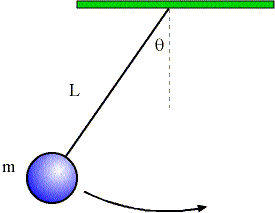
\includegraphics[scale=0.5]{../reviews/review1_fig1}
\end{figure}\\
hanging from a string of length $L$ from a fixed pivot point. When displaced to an initial angle $\theta_{0}$ and released, the pendulum will swing back and forth with periodic motion described by the equation
\[
\theta(t)=\theta_{0}\cos(\sqrt{\frac{g}{L}}t),
\]
where $g$ is the force of gravity and $t$ is the time elapsed since the mass was released. 
\begin{enumerate}
\item	Find an expression for $\theta^{'}(t)$.
\item	Evaluate $\theta^{'}(t)$ at the points $t$ where the displacement is maximized and zero. Interpret your results and provide an intuitive explanation for why these results make sense. 
\end{enumerate}

\end{document}